% !TeX encoding = UTF-8
% !TeX spellcheck = es_ES
% !TeX root = ../ComponentCatalog.tex
%!TEX root=../ComponentCatalog.tex
\begin{table}[H]
    \centering
    \renewcommand\theadfont{\bfseries}
    \setlength{\tabcolsep}{10pt}
    \renewcommand{\arraystretch}{1.5}

    \begin{tabular}{|c|c|c|c|c|}
        \beginConnectorTable{SG-90}
        \multirow{4}{*}{\makecell{SG-90}}
        \connectordata{
            \begin{scope}
                \clip (0,0) rectangle  +(2,1.5);
                \node[inner sep=0pt] at (0.9,0.75)
                    {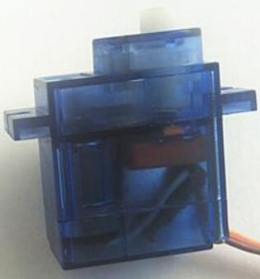
\includegraphics[scale=0.2]{pictures/SG90.jpg}};
            \end{scope}
        }{
            \draw (0,0) rectangle (3,1.5) ;
        }{Aliexpress}{SG-90} {5V} {1A} 
        & \multicolumn{4}{|l|}{\tabitem Sin marca} \\
        \hline
        \connectorblockinfo{Uso}{Control Desvios}
        \connectorblockinfo{Ubicacion}{TT-Tren}
    \end{tabular}
    \caption{Servo SG-90}
    \label{tab:sg90}
\end{table}

\begin{table}[H]
    \centering
    \renewcommand\theadfont{\bfseries}
    \setlength{\tabcolsep}{10pt}
    \renewcommand{\arraystretch}{1.5}

    \begin{tabular}{|c|c|c|c|c|}
        \beginConnectorTable{C1.5CLS}
        \multirow{4}{*}{\makecell{C1.5CLS}}
        \connectordata{
            \begin{scope}
                \clip (0,0) rectangle  +(3,1.5);
                \node[inner sep=0pt] at (1.5,0.75)
                    {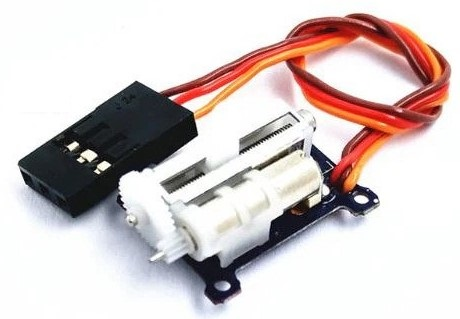
\includegraphics[scale=0.2]{pictures/ServoLineal.jpg}};
            \end{scope}
        }{
            \draw (0,0) rectangle (3,1.5) ;
        }{Aliexpress}{Servo Lineal} {5V} {1A} 
        & \multicolumn{4}{|l|}{\tabitem Sin marca} \\
        \hline
        \connectorblockinfo{Uso}{Control Desvios}
        \connectorblockinfo{Ubicacion}{TT-Tren}
    \end{tabular}
    \caption{Servo SG-90}
    \label{tab:ServoLineal}
\end{table}

\begin{table}[H]
    \centering
    \renewcommand\theadfont{\bfseries}
    \setlength{\tabcolsep}{10pt}
    \renewcommand{\arraystretch}{1.5}

    \begin{tabular}{|c|c|c|c|c|}
        \beginConnectorTable{Controlador}
        \multirow{3}{*}{\makecell{PCA9685}}
        \connectordata{
            \begin{scope}
                \clip (0,0) rectangle  +(3,1.5);
                \node[rotate=1] at (1.5,0.75)
                    {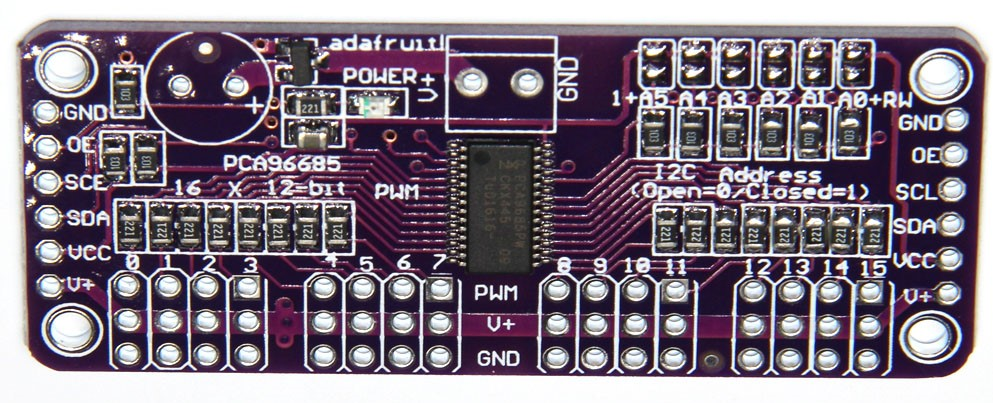
\includegraphics[scale=0.08]{pictures/PCA9685.jpg}};
            \end{scope}
        }{
            \draw (0,0) rectangle (3,1.5) ;
        }{Aliexpress}{PCA9685} {5V} {1A} 
        \hline
        \connectorblockinfo{Uso}{Control Desvios}
        \connectorblockinfo{Ubicacion}{TT-Tren}
    \end{tabular}
    \caption{Servo Controller}
    \label{tab:ServoController}
\end{table}